\documentclass[UTF8]{ctexart}

\usepackage{algorithm}
\usepackage{algorithmic}
\usepackage{amsmath,amssymb}
\usepackage{booktabs}
\usepackage{geometry}
\usepackage{tikz}
\usepackage{color}
\geometry{a4paper,scale=0.7}

\begin{document}
SA22225226 李青航

~\\
\noindent\textbf{254}

Hasse图如下

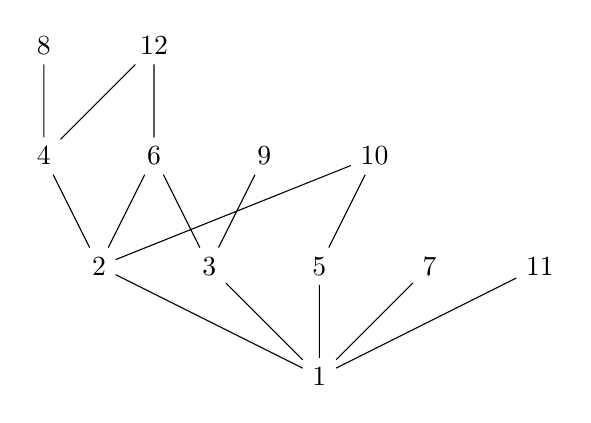
\begin{tikzpicture}[scale=.7][h]
    \node (8) at (-6,6) {$8$};
    \node (12) at (-4,6) {$12$};
    \node (4) at (-6,4) {$4$};
    \node (6) at (-4,4) {$6$};
    \node (9) at (-2,4) {$9$};
    \node (10) at (0,4) {$10$};

    \node (2) at (-5,2) {$2$};
    \node (3) at (-3,2) {$3$};
    \node (5) at (-1,2) {$5$};
    \node (7) at (1,2) {$7$};
    \node (11) at (3,2) {$11$};
    \node (1) at (-1,0) {$1$};
    \draw (1)--(2)--(4)--(8)
          (2)--(6)--(12)
          (4)--(12)
          (1)--(3)--(6)
          (3)--(9)
          (1)--(5)--(10)
          (1)--(7)
          (1)--(11)
          (2)--(10)
          ;

  \end{tikzpicture}

\textbf{i. }

其中一条最大链\{1,2,4,8\}

根据定理5.6.1,最小反链数目是4,其中一种划分是:

$$\{8,12\}$$
$$\{4,6,9,10\}$$
$$\{2,3,5,7,11\}$$
$$\{1\}$$

\textbf{ii. }

其中一条最大反链\{7,8,9,10,11,12\}

根据定理5.6.2 Dilworth定理,最小链数目6,其中一种划分是:

$$\{1,2,4,8\}$$
$$\{3,6,12\}$$
$$\{5,10\}$$
$$\{9\}$$
$$\{7\}$$
$$\{11\}$$

\newpage
\noindent\textbf{257}

设能被4,6,7,10整除的数为$A_1,A_2,A_3,A_4$

$|A_1|=\lfloor 10000/4 \rfloor=2500$

$|A_2|=\lfloor 10000/6 \rfloor= 1666$

$|A_3|=\lfloor 10000/7 \rfloor =1428$

$|A_4|=\lfloor 10000/10 \rfloor =1000$

$|A_1\bigcap A_2|=\lfloor 10000/12 \rfloor=833$

$|A_1\bigcap A_3|=\lfloor 10000/28 \rfloor = 357$

同理算出所有$|A_i\bigcap A_j|$ $|A_i\bigcap A_j \bigcap A_k|$
 $|A_1\bigcap A_2 \bigcap A_3 \bigcap A_4|$


由容斥原理
\begin{equation}
  \nonumber
  \begin{split}
    &
    |\overline{A_1} \bigcap \overline{A_2}
    \bigcap \overline{A_3} \bigcap \overline{A_4}|\\
    &=
    |S|-\sum {|A_i|} +\sum{|A_i \bigcap A_j|}
    -\sum{|A_i\bigcap A_j \bigcap A_k|}
    +{|A_1\bigcap A_2\bigcap A_3\bigcap A_4|}\\
    &=5429
  \end{split}
\end{equation}

~\\
\noindent\textbf{262}

设$A_1$为$\{x|x\in \mathbb{Z}^{+}, x\ge 9\}$,$A_2, A_3,A_4$同理

设$y_1=x_1-9$,$y_2=x_2,y_3=x_3...$转化为$y_1+y_2+y_3+y_4=5$

所以$|A_1|={5+4-1\choose 5}={8 \choose 3}=|A_2|=\dots$

设$y_1=x_1-9,y_2=x_2-9$转化为$y_1+y_2+y_3+y_4=-4$

所以$|A_i\bigcap A_j|=0$

$A_i\bigcap A_j\bigcap A_k$和四项全有的,同理为0

相当于
\begin{equation}
  \nonumber
  \begin{split}
    |\overline{A_1} \bigcap  \overline{A_2} \bigcap  \overline{A_3}  \bigcap \overline{A_4} |
&={17\choose 3}-4{8\choose 3}\\
&=456
  \end{split}
\end{equation}

~\\
\noindent\textbf{264}

设$y_1=x_1-1,y_2=x_2,y_3=x_3-4,y_4=x_4-2$

所以原方程转化为$y_1+y_2+y_3+y_4=13$,其中
$
0\le y_1\le 5,
0\le y_2 \le 7,
0\le y_3,x_4 \le 4
$

设$A_1$为$\{y|y \in \mathbb{Z},y\ge 6 \}$,同理$A_2,A_3,A_4$分别为$y\ge 8,y\ge 5,y\ge 5$

转化为$y_1+y_2+y_3+y_4=13$

设$z_1=y_1-6$,有$z_1+z_2+z_3+z_4=7$
所以$|A_1|={7+4-1\choose 7}$

同理$|A_2|=0$,$|A_3|={8+4-1\choose 8}=|A_4|$

同理再算出所有$|A_i\bigcap A_j|$,$|A_i\bigcap A_j\bigcap  A_k|$,$|A_1\bigcap A_2\bigcap  ...\bigcap A_4|$

用容斥原理,得出结果96

~\\
\noindent\textbf{272}

设$A_1,A_2,A_3$分别表示$aaa,bbbb,cc$出现

则$A_1$表示$\{aaa,4\cdot b,2\cdot c\}$的排列,使用多重集合的排列公式

$$|A_1|=\frac{7}{1!4!2!}=105$$

同理

$$|A_2|=\frac{6}{3!1!2!}=60,|A_3|=\frac{8}{3!4!1!}=280$$

$$|A_1\bigcap A_2|=\frac{4}{1!1!2!}=12,\  |A_1\bigcap A_3|=\frac{6}{1!4!1!=30}$$

$$|A_2|\bigcap A_3|=20,\  |A_1\bigcap A_2 \bigcap A_3|=6$$

所以
\begin{equation}
  \nonumber
  \begin{aligned}
    |\overline{A_1} \cap \overline{A_2} \cap \overline{A_3}| =& |S| - \sum |A_i| + \sum |A_iA_j| - \sum|A_iA_jA_k| \\
    =& 1260 - (105+60+280) +(12+30+20) - 6 \\
    =& 871
    \end{aligned}
\end{equation}


~\\
\noindent\textbf{279}

\textbf{(a)  }

设$r_k$为$k$个禁止位上摆放棋子的方法数

显然$$r_0=1,     r_1=6$$

将禁止位分三部分,每一部分最多只能放置一辆车,用乘法原理
$$r_2= \dbinom{3}{2} \times 2^2 = 12$$

$$r_3 = \dbinom{3}{3}\times 2^3 = 8$$

禁止位置上无法摆放四辆及以上的车,因此,$r_i = 0, i \ge 4$

所以总的方法数为
$$\sum_{k=0}^{n} r_k (-1)^k (n-k)! = 1 \times 6! - 6 \times 5! + 12 \times 4! - 8 \times 3! = 240$$

\newpage
\textbf{(b)  }

同理$$r_0=1,     r_1=12$$

将禁止位分三部分,每一部分最多只能放置2辆车,用乘法原理

一部分放2个车,每部分2种放法,3个部分,所以$2\times 3$;
加上 一部分放一个车,3部分选2部分放车,每部分4种放法,${3\choose 2}\times 4^2$
$$
r_2=2\times 3 +{3\choose 2}\times{4^2}=54
$$

3车放三部分,分为一一一和二一零,两种方法,加法原理。
$$
r_3=4^3+3!\times 2 \times 4=112
$$

4车放三部分,分为二二零,二一一
$$
r_4={3\choose 2}\times 2^2 + {3\choose 1}\times 4^2 \times 2=108
$$

5车放三部分,只能二二一
$$
r_5={3\choose 1}\times 2^2 \times 4=48
$$

6车放三部分,只能二二二
$$
r_6=2^3=8
$$

禁止位置上无法摆放7个及以上的车,因此$r_i = 0, i \ge 7$

总的摆放数
\begin{equation}
  \nonumber
  \begin{split}
\sum_{k=0}^{n} r_k (-1)^k (n-k)!&=
1 \times 6! - 12 \times 5! + 54 \times 4! 
- 112 \times 3! + 108 \times 2! - 48 
\times 1! + 8 \times 0!\\
&= 80
  \end{split}
\end{equation}

\textbf{(c)  }

将棋盘禁止位分为相互独立的$F_1$和$F_2$,
分别求出$F_1$和$F_2$能摆放车的方法数,如下表

\begin{table}[h]
  \centering
  \begin{tabular}{c|cccc} 
  \hline
  $k$       & 0 & 1 & 2 & 3  \\ 
  \hline
  $F_1(k)$ & 1 & 5 & 6 & 1  \\
  \hline
  \end{tabular}

  \begin{tabular}{c|ccc} 
    \hline
    $k$       & 0 & 1 & 2   \\ 
    \hline
    $F_2(k)$ & 1 & 3 & 1   \\
    \hline
    \end{tabular}
\end{table}

总的,使用乘法原理与加法原理
$$r_k = \sum_{j=0}^{k} F_1(j) F_2(k-j)$$


\begin{table}[h]
  \centering
  \begin{tabular}{c|ccccccc} 
  \hline
  $k$    & 0 & 1 & 2  & 3  & 4 & 5 & 6  \\ 
  \hline
  $r_k$ & 1 & 8 & 22 & 24 & 9 & 1 & 0  \\
  \hline
  \end{tabular}
\end{table}

所以总的方法数为

\begin{equation}
  \nonumber
  \begin{aligned}
    \sum_{k=0}^{n} r_k (-1)^k (n-k)! &=
     1 \times 6! - 8 \times 5! + 22 \times 4!
      - 24 \times 3! + 9 \times 2! - 1 \times 1! 
      + 0 \times 0!\\
      &= 161
  \end{aligned}
\end{equation}

~\\
~\\
~\\
\underline{下一页还有}\\
\underline{下一页还有}\\
\underline{下一页还有}\\

\newpage
\noindent\textbf{281}

转化为棋盘放车问题

\begin{table}[h]
  \centering
  \begin{tabular}{|l|l|l|l|l|l|} 
  \hline
  $\boxtimes$ & $\boxtimes$ & $\boxtimes$ & ~~~~&                              &                                \\ 
  \hline
  $\boxtimes$ &                               &                               &  &                               &                                \\ 
  \hline
  $\boxtimes$ &                               &                               &  &                               &                                \\ 
  \hline
                                &                               &                               &  &                               &                                \\ 
  \hline
                                &                               &                               &  & $\boxtimes$ & $\boxtimes$  \\ 
  \hline
                                &                               &                               &  & $\boxtimes$ & $\boxtimes$  \\
  \hline
  \end{tabular}
  \end{table}

对于每一部分,先计算摆放车可能的种类数

\begin{table}[h]
    \centering
    \begin{tabular}{c|cccc} 
    \toprule
    $k$     & 0 & 1 & 2 & 3  \\
    $F_1(k)$ & 1 & 5 & 4 & 0  \\
    \bottomrule
    \end{tabular}

    \begin{tabular}{c|cccc}
      \toprule
      $k$     & 0 & 1 & 2 & 3  \\
      $F_2(k)$ & 1 & 4 & 2 & 0  \\
      \bottomrule
      \end{tabular}

\end{table}

总的种类,见表1
$$r_k = {\sum_{i=0}^{n} F_1(i)} \times F_2(k-i)$$

\begin{table}[h]
  \centering
  \caption{281题 $r_i$}
  \begin{tabular}{c|ccccccc} 
  \toprule
  $k$ & 0 & 1 & 2  & 3  & 4 & 5 & 6  \\
  $r_k$ & 1 & 9 & 26 & 26 & 8 & 0 & 0  \\
  \bottomrule
  \end{tabular}
  \end{table}

总数
$$
\sum_{k=0}^{n} r_k (-1)^k (n-k)! =
1 \times 6! - 9 \times 5! + 26 \times 4! - 26 \times 3! + 8 \times 2! = 124
$$
\end{document}